\documentclass[a4paper, 12pt, twoside]{report}

\usepackage{fontspec}
\usepackage{xunicode}
\usepackage{xltxtra}
\usepackage{xgreek}
\usepackage{csquotes}
\usepackage{hyperref}
\usepackage{placeins}

\raggedbottom
\onecolumn

\usepackage{graphicx, amsfonts, psfrag, fancyhdr, layout, subfigure}
\usepackage{pdflscape}
%\usepackage{lscape}
\usepackage{multirow}
\usepackage{longtable}
\usepackage{array}
%The arydshln package offers you the \hdashline and \cdashline commands which are the dashed counterparts of \hline and \cline, respectively. 
\usepackage{arydshln}

\usepackage[toc,page]{appendix}
\renewcommand{\appendixtocname}{Παραρτήματα}
\renewcommand{\appendixname}{Παράρτημα}
\renewcommand{\appendixpagename}{Παραρτήματα}

\setmainfont[Mapping=tex-text]{GFS Artemisia}

\usepackage[style=numeric, bibstyle=numeric, hyperref=true, backref=true, alldates=terse, indexing=false, backend=bibtex]{biblatex}
\addbibresource{Bibliography.bib}

\usepackage{index}
\usepackage[columns=2]{idxlayout}
\newindex{default}{idx}{ind}{Ευρετήριο}

% Set equal margins on book style
\setlength{\oddsidemargin}{53pt}
\setlength{\evensidemargin}{53pt}
\setlength{\marginparwidth}{57pt}
\setlength{\footskip}{30pt}

\author{Καφετζής Δημήτριος Ανδρέας}
\title{Εναέρια λήψη εικόνας - Πρώτη τεχνική έκθεση : Μελέτη σύστασης/κατασκευής πλήρους συστήματος εναέριας λήψης εικόνας}

\begin{document}
	
	\maketitle
	
	\section*{Περίληψη}
		\paragraph{}{Με την αναφορά αυτή επιχειρείται να αποσαφηνιστεί το ίδιο το σύστημα της εναέριας λήψης εικόνας. Παρουσιάζονται τα επί μέρους τμήματα και προτείνονται λύσεις.
		}
		
	\addcontentsline{toc}{chapter}{Περιεχόμενα}
	\tableofcontents

	\newpage
	\phantomsection
	\addcontentsline{toc}{chapter}{Κατάλογος Σχημάτων}
	\listoffigures

	\newpage
	\phantomsection
	\addcontentsline{toc}{chapter}{Κατάλογος Πινάκων}
	\listoftables
	
% Code for creating empty pages
% No headers on empty pages before new chapter
	\makeatletter
		\def\cleardoublepage{
			\clearpage\if@twoside \ifodd\c@page\else
	    	\hbox{}
	    	\thispagestyle{plain}
	    	\newpage
    		\if@twocolumn\hbox{}\newpage\fi\fi\fi
    	}
	\makeatother \clearpage{\pagestyle{plain}\cleardoublepage}

% Define pagestyle
	\pagestyle{fancy}
	\fancyhf{}
	\renewcommand{\chaptermark}[1]{\markboth{ \emph{#1}}{}}

% Adjustments headers
	\fancyhead[LO]{\emph{Κεφάλαιο \thechapter}}
	\fancyhead[RE]{\leftmark}
	\fancyfoot[LE,RO]{\thepage}
	
	\chapter{Εισαγωγή}
		
		\section{Σκοπός}
			\paragraph{}{Σκοπός μας είναι η σύνθεση και κατασκευή ενός συστήματος εναέριας λήψης φωτογραφιών και βίντεο υψηλής ανάλυσης σε ποικίλες καιρικές συνθήκες. Τα συστήματα αυτά χαρακτηρίζονται ως μη επανδρωμένες εναέριες μηχανές (Uav, Unmanned aerial vehicle)
			}
			
		\section{Γενικές απαιτήσεις}
			\paragraph{}{Η κατασκευή και η λειτουργία του συστήματος θα πρέπει να γίνει λαμβάνοντας υπόψιν τους παρακάτω παραμέτρους :
				\begin{itemize}
					\item Ασφάλεια - εξοπλισμού και περιβάλλοντος
					\item Ευχρηστία – πτήσης και λήψης εικόνας
					\item Λειτουργικότητα – πτήσης και λήψης εικόνας
					\item Ποιότητα – εξοπλισμού, πτήσης και λαμβανόμενης εικόνας
					\item Διάρκεια – πτήσης και λαμβανόμενης εικόνας
Κόστος
				\end{itemize}
			}
			
			\paragraph{Ασφάλεια}{Το σύστημα θα πρέπει να είναι ασφαλές, αφενός για τον εαυτό του με σκοπό την προστασία του εξοπλισμού και την αποφυγή καταπόνησης του και αφετέρου για τους χρήστες και το ευρύτερο περιβάλλον στο οποίο θα λειτουργεί.

 			\paragraph{Ευχρηστία}{Το σύστημα όντας εύχρηστο θα μας απαλλάξει από δυσάρεστες καταστάσεις. Απαιτούμενος σκοπός είναι η πτήση και η λήψη εικόνας να γίνονται όσο το δυνατόν ομαλά και ευχάριστα για τους χειριστές. Η εμπλεκόμενες διαδικασίες θα πρέπει να είναι αυτοματοποιημένες σε μεγάλο βαθμό δίνοντας τη δυνατότητα στους χειριστές να επικεντρωθούν στην ποιότητα του τελικού αποτελέσματος.

 			\paragraph{Λειτουργικότητα}{Θα πρέπει να παρέχονται οι κατάλληλες προϋποθέσεις στους χειριστές του συστήματος για την παραγωγή υψηλής ποιότητας εικόνας και μεγάλου αισθητικού ενδιαφέροντος.

 			\paragraph{Ποιότητα}{Ο παράγοντας αυτός αφορά τόσο τα κατασκευαστικά χαρακτηριστικά του εξοπλισμού, όσο και την ποιότητα της πτήσης και της καταγραφόμενης εικόνας. Ο εξοπλισμός οφείλεται να αντέξει στο χρόνο με εμφάνιση ελαχίστων προβληματικών εξαρτημάτων ή υποσυστημάτων και με διακριτική συντήρηση τους. Επιπλέον, η πτήση αναμένεται να είναι τόσο ομαλή και ανεπηρέαστη από τις διάφορες καιρικές συνθήκες (αέρας, βροχή, χιόνι) ώστε να αποτελεί αιτία για λήψη χαμηλής ποιότητας φωτογραφιών και βίντεο. Αναφορικά με την ίδια την ποιότητα της λαμβανόμενης εικόνας επιθυμείτε να είναι η μέγιστη δυνατή αν όχι υψηλής ανάλυσης (high definition).

 			\paragraph{Διάρκεια}{Το σύστημα θα πρέπει να επιτρέπει την αδιάλειπτη καταγραφή εικόνας για μεγάλο χρονικό διάστημα. Ως ενδεικτικός χρόνος συνεχόμενης πτήσης αναφέρονται τα σαράντα (40) λεπτά, ενώ για το χρόνο καταγραφής οι δύο (2)  με δυόμιση (2 και 1/2) ώρες.

 			\paragraph{Κόστος}{Το κόστος απαιτείται να κυμανθεί στο χαμηλότερο δυνατό επίπεδο. Η σύσταση του συστήματος οφείλεται να γίνει λαμβάνοντας υπόψιν τον υπάρχων εξοπλισμό.
 			
 	\chapter{Τεχνική ανάλυση}
		\section{Εισαγωγή}
			\paragraph{}{Στο κεφάλαιο αυτό θα παρουσιάσουμε τα μέρη από τα οποία θα αποτελείται το σύστημα. Θα καταγραφούν τα χαρακτηριστικά που πρέπει να έχει το κάθε τμήμα του ώστε να πληρούνται οι απαιτήσεις που τέθηκαν στο προηγούμενο κεφάλαιο.
			}
			
			\paragraph{}{Ας ξεκαθαρίσουμε από τι μέρη θα αποτελείται το εν λόγω σύστημα.
			\begin{itemize}
				\item πλατφόρμα πτήσης
				\item πλατφόρμα προσγείωσης
				\item αυτόματος πιλότος
				\item χειροκίνητη πτήση
				\item επίγειος σταθμός ελέγχου πτήσης
				\item πλατφόρμα της μηχανής
				\item αυτόματος πιλότος για πλατφόρμα της μηχανής
				\item μηχανή
				\item επίγειος σταθμός ελέγχου της μηχανής
				\item εναέριος σταθμός μετάδοσης εικόνας
				\item επίγειος σταθμός λήψης σύγχρονης εικόνας
				\item επίγειος σταθμός καταγραφής της εικόνας
			\end{itemize}
			}
		
		
		\section{Πτητική μηχανή}
		\subsection{Πλατφόρμα πτήσης και προσγείωσης}
			\paragraph{πλατφόρμα πτήσης}{Αναφέρεται στην πτητική συσκευή. Για λόγους ευστάθειας, ασφάλειας, ευχρηστίας, συντήρησης οδηγούμαστε στην επιλογή ενός ηλεκτρικού μέσου και συγκεκριμένα ενός πολυπτέρου. Το πλήθος των κινητήρων δεν έχει αποσαφηνιστεί. Επιλογές αποτελούν τα εξάπτερα και τα οχτάπτερα.
			}
			\paragraph{}{Κάθε πολύπτερο απαρτίζεται από τον σκελετό, τους κινητήρες, τους ελεγκτές των κινητήρων και τους έλικες. Στην αγορά διατίθενται μοντέλα που περιλαμβάνουν όλα αυτά τα υποσυστήματα και μοντέλα που αποτελούνται μόνο από το σκελετό δίνοντας την ευελιξία για την χρήση κινητήρων της επιλογής μας. Για τα τελευταία μοντέλα θα χρειαστεί η συμβουλή και η πιθανότητα η συναρμολόγηση τους από ειδικό πάνω στον
			}
			\paragraph{}{Η πλατφόρμα αυτή μαζί με τη βάση για τη μηχανή αποτελούν τα κυριότερα υποσυστήματα αφού θα καθορίσουν και την επιλογή των υπολοίπων. Στα βασικά χαρακτηριστικά της πτητικής πλατφόρμας πρέπει να περιλαμβάνονται η εύκολη και γρήγορη συναρμολόγηση της, η ανύψωση όσο το δυνατόν μεγαλύτερου φορτίου, η προστασία του περιβάλλοντος της από τους περιστρεφόμενους έλικες. Επιπλέον, η μεγαλύτερη δυνατή παρουσία στον αέρα και αντιμετώπιση διαφορετικών καιρικών συνθηκών αποτελούν σημαντικοί παράγοντες.
			}			
			\paragraph{πλατφόρμα προσγείωσης}{Αναφέρεται στα "πόδια" του συστήματος. Συνήθως αποτελούν ενιαίο τμήμα με την πλατφόρμα πτήσης.
			}
			\paragraph{}{Οι εταιρίες που δραστηριοποιούνται στο χώρο των πολυπτέρων διαθέτουν όλες τους μοντέλα που ικανοποιούν επί το πλείστον τις απαιτήσεις μας. Έχουν ικανοποιητική δύναμη για να ανυψώσουν το βάρος όλου του συστήματος, συναρμολογούνται μέσα σε 5 με 10 λεπτά και μπορούν να συντηρηθούν εύκολα και γρήγορα. Επιπλέον, τα προτεινόμενα συστήματα υποστηρίζονται συνεχώς από τις κατασκευάστριες εταιρίες με αποτέλεσμα να διορθώνονται τυχόν δυσλειτουργίες, να παρουσιάζονται αναβαθμίσεις παρουσιάζονται και να μην υπάρχει έλλειψη ανταλλακτικών.
			}
			\paragraph{}{Από τα απαιτούμενα χαρακτηριστικά κανένα από τα προτεινόμενα μοντέλα δεν διαθέτει σύστημα προστασίας από τους περιστρεφόμενους έλικες. Γενικά η αγορά υπολείπεται στον τομέα αυτό. Έχουν υπάρξει κάποιες προσπάθειες αλλά δεν αποτελούν αξιόπιστη λύση. Η μόνη εν αναμονή λύση προέρχεται από την εταιρία Safeflight Copters\footnote{ιστοσελίδα : \url{http://safeflightcopters.com/}}. Δυστυχώς όμως δεν έχει φτάσει ακόμα στο στάδιο της διάθεσης.
			}
			\paragraph{}{Τέλος, μόνο η εταιρία Droidworx προσφέρει σύστημα προστασίας του εξοπλισμού. Συγκεκριμένα στο πάνω μέρος της πλατφόρμας τοποθετούνται προστατευτικές μπάρες ή προστατευτικό κάλυμμα, το οποίο κάλυμμα προφυλάσσει και από βροχή.
			}
			
		\subsubsection{Εξάπτερα μοντέλα}
			\paragraph{}{Στον πίνακα \ref{πιν.:Μοντέλα εξαπτέρων} παρουσιάζονται τα προτεινόμενα μοντέλα.
			}
			\paragraph{DJI Spreading Wings S800}{Εξάπτερο της εταιρίας DJI που ενσωματώνει και το σύστημα προσγείωσης. Κεντρικό εξάρτημα αποτελεί η κεντρική πλατφόρμα στην οποία ενσωματώνονται τα υπόλοιπα συστήματα. Διαθέτει και ειδικό χώρο για την IMU μονάδα του αυτόματου πιλότου της ίδιας της εταιρίας. Επιπλέον, οι βραχίονες έχουν ενσωματωμένους τα κυκλώματα οδήγησης των κινητήρων και τα απαραίτητα καλώδια. Γενικά, αποτελεί μία στιβαρή κατασκευή, με αρκετά προσεγμένο σχεδιασμό και οργανωμένη διάταξη των εξαρτημάτων.
			}
			\paragraph{}{Παρατίθενται δείγματα δουλειάς του συγκεκριμένου εξαπτέρου :
				\begin{itemize}
					\item \href{http://www.youtube.com/watch?v=PXCc_1IqXW4}{DJI video 1}
					\item \href{http://www.youtube.com/watch?v=GldKyaEqlUA}{DJI S800- quick installation video}
					\item \href{http://www.youtube.com/watch?v=zr1npAPBLEo}{DJI S800 - stationary flight}
					\item \href{https://vimeo.com/44573759}{DJI Z15 carrying a Sony Nex 5n mounted on a DJI S800}
					\item \href{https://vimeo.com/48097149}{dji s800 hexacopter with zenmuse head and sony nex-5n}
				\end{itemize}
			}
			\begin{figure}[hp]
					\centering
					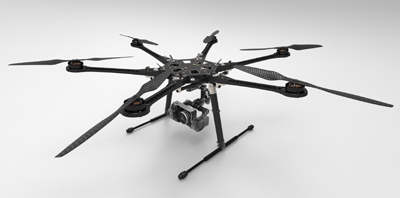
\includegraphics[scale=0.50]{DJI_S800.png}
					\caption{DJI Spreading Wings S800 \href{http://www.dji-innovations.com/wp-content/uploads/2012/05/S800_1.jpg}{[πηγή]}}
					\label{φωτ:DJI Spreading Wings S800}
			\end{figure}
			
			
			\paragraph{FreeFly Cinestar 6}{Εξάπτερο της Freefly Systems με χαρακτηριστικά την εύκολη συναρμολόγηση και την προσοχή που έχει δοθεί στη σταθερότητα του, δηλαδή στη μείωση της δόνησης που δέχεται το σύστημα της φωτογραφικής μηχανής.
			}
			\paragraph{}{Παρατίθενται δείγματα δουλειάς του συγκεκριμένου εξαπτέρου :
				\begin{itemize}
					\item \href{http://www.youtube.com/watch?v=Yo6Wdmt1zSU}{DJI video 1}
					\item \href{http://www.youtube.com/watch?v=t4ZkjpicWuo}{Payload test}
					\item \href{http://www.youtube.com/watch?v=fs1EynZ3E8o}{Cinestar 6 and Cinestar gimbal}
					\item \href{http://www.youtube.com/watch?v=J9hA6OfK9mE}{Cinestar 6}
					\item \href{http://www.youtube.com/watch?v=Bq6r-Ex6z98}{Cinestar 6 above Nab2012}
					\item \href{https://vimeo.com/47171190}{FreeFly Radian Stabiliser/Cinestar 6/Photohigher Av130/Panasonic GH2}
				\end{itemize}
			}
			\begin{figure}[hp]
					\centering
					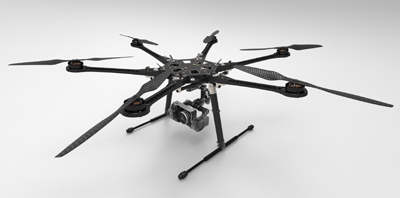
\includegraphics[scale=0.50]{DJI_S800.png}
					\caption{Cinestar 6 \href{http://www.freeflysystems.com/images/products/cinestar-6-detail.png}{[πηγή]}}
					\label{φωτ:Cinestar 6}
			\end{figure}

			\paragraph{Droidworx AD-6HL}{Εξάπτερο της Droidworx φτιαγμένο από ανθρακονήματα και σχεδιασμένο για ανύψωση αυξημένου φορτίου. Συνδυάζεται με αρκετά συστήματα αυτόματων πιλότων και παρέχει τη δυνατότητα για 360 μοίρες θέαση με το να υποστηρίζει πλατφόρμες φωτογραφικής μηχανής που ενσωματώνουν το σύστημα προσγείωσης. Όσον αφορά τις υποστηριζόμενες μηχανές αυτές είναι οι Samsung HMX-Q10, Panasonic GH2 και Canon 550d. 
			}
			\paragraph{Droidworx Skyjib 6}{Εξάπτερο της Droidworx όπως και το προηγούμενο, αλλά αποτελεί το μεγαλύτερο πολύπτερο της εταιρίας. Είναι κατασκευασμένο για να σηκώνει μέχρι και 10 κιλά (π.χ. τη μηχανή Red Epic) διατηρώντας τα υπόλοιπα πλεονεκτήματα του προηγούμενου μοντέλου.
			}
			\paragraph{}{Ένα βασικό πλεονέκτημα των δυο παραπάνω μοντέλων αποτελεί το προστατευτικό κάλυμμα το οποίο μπορεί να τοποθετηθεί στο πάνω μέρος της πλατφόρμας πτήσης.
			}
			\paragraph{}{Παρατίθενται δείγματα δουλειάς των συγκεκριμένων εξαπτέρων :
				\begin{itemize}
					\item \href{http://vimeo.com/moogaloop.swf?clip_id=29893580&server=vimeo.com&show_title=1&show_byline=1&autoplay=1}{Droidworx AD-6HLE - Hexaprod Promo Video}
					\item \href{https://vimeo.com/20411633}{Panasonic GH2 on Droidworx AD-6 Hexakopter}
					\item \href{https://vimeo.com/20921788}{FPV flight with AD6 and Panny GH2 over Steamboat Lake}
					\item \href{https://vimeo.com/42030489}{SkyJib 6X flying Red}
					\item \href{https://vimeo.com/25265975}{Droidworx CS series - flight testing}
				\end{itemize}
			}
			\begin{figure}[hp]
					\centering
					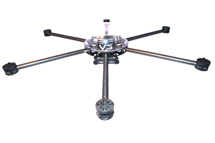
\includegraphics[scale=0.50]{Droidworx_AD_6HL.png}
					\caption{Droidworx AD-6HL \href{http://www.droidworx.com.au/shop/components/com_virtuemart/shop_image/product/AD_6_Heavy_Lift__4e2f78f506a46.jpg}{[πηγή]}}
					\label{φωτ:Droidworx AD-6HL}
			\end{figure}
			\begin{figure}[hp]
					\centering
					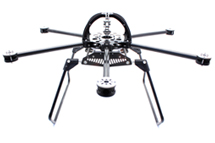
\includegraphics[scale=0.50]{Droidworx_skyjib6.png}
					\caption{Droidworx SkyJib 6 \href{http://www.droidworx.com.au/shop/components/com_virtuemart/shop_image/product/SkyJib_6_for_Ret_4f1e21acba3d6.jpg}{[πηγή]}}
					\label{φωτ:SkyJib 6}
			\end{figure}
			
			\begin{landscape}	
			\setlength\LTleft{0pt}            % default: \parindent
			\setlength\LTright{0pt}           % default: \fill
	
			\begin{longtable} { m{3cm} m{3.5cm} m{3.5cm} m{3.5cm} m{3.5cm} }
					\caption [Μοντέλα εξαπτέρων]{Μοντέλα εξαπτέρων}
					\label{πιν.:Μοντέλα εξαπτέρων}\\
					\hline
					\endfirsthead
					\multicolumn{5}{c}{συνέχεια του πίνακα \ref{πιν.:Μοντέλα εξαπτέρων}}\\
					\hline
					~\\
					\endhead
					\hline
					\multicolumn{5}{c}{ο πίνακας συνεχίζεται στην επόμενη σελίδα}\\
					\endfoot
					\multicolumn{5}{c}{ολοκληρώθηκε ο πίνακας \ref{πιν.:Μοντέλα εξαπτέρων}}\\
					\endlastfoot
					~\\
					Μοντέλο & DJI Spreading Wings S800 & Cinestar 6 & AD-6HL & SkyJib 6\\
					\hdashline
					~\\
					Κατασκευαστής & DJI Innovations & FreeFly Systems & Droidworx & Droidworx\\
					Ιστοσελίδα & \href{http://www.dji-innovations.com/products/spreading-wings-s800/overview/}{dji-innovations} & \href{http://www.freeflysystems.com/products/cinestar-6.php}{FreeFly Systems} & \href{http://www.droidworx.com.au/ADseries.html}{Droidworx} & \href{http://www.droidworx.com.au/skyjib.html}{Droidworx}\\
					\hdashline
					~\\
					\multicolumn{5}{c}{Χαρακτηριστικά}\\
					\hdashline
					βάρος απογείωσης (κιλά) & 5-7 & 5,8 (μέγιστο) & 4,2 & 6,6\\
					~\\
					βάρος φορτίου -πλατφόρμας και gimbal (κιλά) & 0-2,5 & 2,6 & 1,75 & 3\\
					~\\
					μπαταρίες & LiPo (6S, 10000mAh~15000mAh, 15C(Min)) & & & \\
					~\\
					μέγιστη κατανάλωση (watt) & 2100W & & & \\
					~\\
					κατανάλωση αιώρησης (watt) & 720W (με 6 κιλά βάρος) & & & \\
					~\\
					μέγιστος χρόνος αιώρησης (λεπτά) & 16 λεπτά (@10000mAh \& 6κιλά βάρος) & & & \\
					~\\
					τάση τροφοδοσίας κινητήρων & 6S LiPo & & & \\
					υποστηριζόμενες μηχανές  & Nex5-7, Panasonic GH2 & a GoPro to a Red Epic & Samsung HMX-Q10, Panasonic GH2, Canon 550d & Up to Red Scarlet class camera\\
					προτεινόμενα gimbal & Zenmuse Z15 & cinestar 3-axis & AV-200/360 - AV130/360 & AV200\\
					\hline
				\end{longtable}
				\end{landscape}
			
		\subsubsection{Οχτάπτερα}

			\paragraph{}{Στον πίνακα \ref{πιν.:Μοντέλα οχταπτέρων} παρουσιάζονται τα προτεινόμενα μοντέλα.
			}
			\paragraph{}{χχχ
			}
			\paragraph{}{Παρατίθενται δείγματα δουλειάς του συγκεκριμένου οχταπτέρου :
				\begin{itemize}
					\item \href{χχχχ}{χχχχ}
				\end{itemize}
			}
%			\begin{figure}[hp]
%					\centering
%					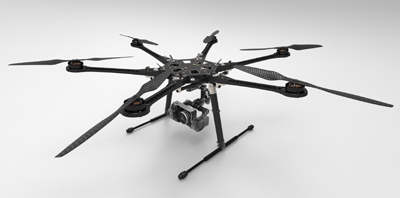
\includegraphics[scale=0.50]{DJI_S800.png}
%					\caption{DJI Spreading Wings S800 \href{http://www.dji-innovations.com/wp-content/uploads/2012/05/S800_1.jpg}{[πηγή]}}
%					\label{φωτ:DJI Spreading Wings S800}
%			\end{figure}

			\begin{landscape}	
			\setlength\LTleft{0pt}            % default: \parindent
			\setlength\LTright{0pt}           % default: \fill
	
			\begin{longtable} { m{3cm} m{3.5cm} m{3.5cm} m{3.5cm} }
					\caption [Μοντέλα οχταπτέρων]{Μοντέλα οχταπτέρων}
					\label{πιν.:Μοντέλα οχταπτέρων}\\
					\hline
					\endfirsthead
					\multicolumn{4}{c}{συνέχεια του πίνακα \ref{πιν.:Μοντέλα οχταπτέρων}}\\
					\hline
					~\\
					\endhead
					\hline
					\multicolumn{4}{c}{ο πίνακας συνεχίζεται στην επόμενη σελίδα}\\
					\endfoot
					\multicolumn{4}{c}{ολοκληρώθηκε ο πίνακας \ref{πιν.:Μοντέλα οχταπτέρων}}\\
					\endlastfoot
					~\\
					Μοντέλο & Cinestar 8 & Droidworx AD8 V3 & SkyJib 8\\
					\hdashline
					~\\
					Κατασκευαστής &  &  &\\
					Ιστοσελίδα &  & &\\
					\hdashline
					~\\
					\multicolumn{4}{c}{Χαρακτηριστικά}\\
					\hdashline
					βάρος απογείωσης (κιλά) &  &  &\\
					~\\
					βάρος φορτίου -πλατφόρμας και gimbal (κιλά) &  &  &\\
					~\\
					μπαταρίες & & &\\
					~\\
					μέγιστη κατανάλωση (watt) & & &\\
					~\\
					κατανάλωση αιώρησης (watt) & & &\\
					~\\
					μέγιστος χρόνος αιώρησης (λεπτά) & & &\\
					~\\
					τάση τροφοδοσίας κινητήρων & & &\\
					υποστηριζόμενες μηχανές  & & & \\
					προτεινόμενα gimbal & & &\\
					\hline
				\end{longtable}
				\end{landscape}	
			
		\subsection{Αυτόματος πιλότος και χειριστήριο εδάφους}
			\paragraph{αυτόματος πιλότος}{Για την εξασφάλιση τόσο της ασφάλειας πολυπτέρου και περιβάλλοντος, όσο και της ποιότητας του αποτελέσματος κρίνεται απαραίτητος. Διαθέτοντας αυτόν, το πολύπτερο μπορεί να αιωρείται μόνο του χωρίς την παρέμβαση του ανθρώπου από το έδαφος, ελαχιστοποιώντας με αυτόν τον τρόπο τις αναταράξεις που μπορεί να επιφέρει η χειροκίνητη καθοδήγηση. Επίσης, σημαντικό αποτελεί το γεγονός ότι χάνοντας το σήμα δεν καταρρίπτεται αλλά διατηρεί το ύψος ή/και την πορεία του. Επιπλέον, δύναται να προγραμματιστεί ώστε να επιστρέφει αυτόματα ύστερα από κάποια δεύτερα. Τέλος, στο ίδιο μοτίβο, σε περίπτωση που οι μπαταρίες αδειάσουν, επιστρέφει σε προκαθορισμένο σημείο προσγείωσης με ασφάλεια.
			}
			\paragraph{}{Υπάρχουν εταιρίες που προσφέρουν ολοκληρωμένα συστήματα αυτόματου πιλότου τα οποία διαφοροποιούνται στην ποιότητα τους -στο πόσο σταθερό είναι το πολύπτερο στον αέρα- και στις λειτουργίες που ενσωματώνουν δίνοντας ιδιαίτερη έμφαση στην αυτόματες διαδικασίες ασφάλειας.
			}
			\paragraph{}{Στον πίνακα \ref{πιν.:Μοντέλα αυτόματων πιλότων} παρουσιάζονται τα προτεινόμενα μοντέλα.
			}
			
			\paragraph{Zero YS-X6}{Παρατίθενται δείγματα δουλειάς του συγκεκριμένου πιλότου :
				\begin{itemize}
					\item \href{http://www.youtube.com/watch?v=r1_O_VvFZ1U}{Zero YS-X6 10km/h test}
					\item \href{http://www.youtube.com/watch?v=JRiiGby-e-4}{Zero YS-X6}					
				\end{itemize}
			}
			
			\paragraph{DJI Wookong-M}{Αποτελεί ένα πλήρες σύστημα αυτοματοποιημένης πτήσης. Διαθέτει τρία mode πτήσης. Το Gps-Atti όντας απόλυτα αυτόματο από την απογείωση μέχρι και την προσγείωση ή το Atti το οποίο αφορά χειροκίνητο χειρισμό με ενεργοποιημένο το σταθεροποιητή πτήσης και τέλος την πλήρως χειροκίνητη πτήση χωρίς καμία βοήθεια.
			}
			\paragraph{}{Παρατίθενται δείγματα δουλειάς του συγκεκριμένου πιλότου :
				\begin{itemize}
					\item \href{https://vimeo.com/38972821}{DJI Wookong-M}
					\item \href{https://vimeo.com/43035644}{Droidworx ADX3 HL, DJI Wookong}
					\item \href{https://vimeo.com/40803086}{DJI Wookong 4S Test 1}			
				\end{itemize}
			}
			
			\paragraph{Feiyu Tech FY-91Q}{Ο συγκεκριμένος πιλότος έχει ως μεγάλο πλεονέκτημα την τιμή του, αλλά δυστυχώς δεν διαθέτει αρκετές λειτουργίες καθώς και μονάδα τροφοδοσίας. Παρατίθενται δείγματα δουλειάς του συγκεκριμένου πιλότου :
				\begin{itemize}
					\item \href{https://vimeo.com/27469866}{FY91Q Kiso river}
					\item \href{http://www.youtube.com/watch?v=5JWZVufFHKQ}{FY-91Q GoPro}
				\end{itemize}
			}
			
			\paragraph{HoverflyPRO}{Παρατίθενται δείγματα δουλειάς του συγκεκριμένου πιλότου :
				\begin{itemize}
					\item \href{https://vimeo.com/26895602#}{Guam helicopter aerials}
					\item \href{http://www.youtube.com/watch?v=b0fwnqsdI8w}{Aerial Video - Aspen Trees}
					\item \href{https://vimeo.com/29466533#}{Got Aerial and Aerial Exposure}
				\end{itemize}
			}
			
			\begin{landscape}	
			\setlength\LTleft{0pt}            % default: \parindent
			\setlength\LTright{0pt}           % default: \fill
	
			\begin{longtable} { m{3cm} m{3.5cm} m{3.5cm} m{3.5cm} m{3.5cm} }
					\caption [Μοντέλα αυτόματων πιλότων]{Μοντέλα αυτόματων πιλότων}
					\label{πιν.:Μοντέλα αυτόματων πιλότων}\\
					\hline
					\endfirsthead
					\multicolumn{5}{c}{συνέχεια του πίνακα \ref{πιν.:Μοντέλα αυτόματων πιλότων}}\\
					\hline
					~\\
					\endhead
					\hline
					\multicolumn{5}{c}{ο πίνακας συνεχίζεται στην επόμενη σελίδα}\\
					\endfoot
					\multicolumn{5}{c}{ολοκληρώθηκε ο πίνακας \ref{πιν.:Μοντέλα αυτόματων πιλότων}}\\
					\endlastfoot
					~\\
					Μοντέλο & Zero YS-X6 GU-INS & DJI Wookong-M & Feiyu Tech FY-91Q & HoverflyPRO\\
					\hline
					~\\
					Κατασκευαστής & Zero & DJI Innovations & Feiyu Tech & Hoverfly\\
					Ιστοσελίδα & \href{http://www.zerouav.net/productmore.aspx?id=82}{Zero} & \href{http://www.dji-innovations.com/products/wookong-m/overview/}{dji-innovations} & \href{http://www.feiyu-tech.com/product-en.php?id=12&mlist=3&}{Feiyu Tech} & \href{http://www.feiyu-tech.com/product-en.php?id=12&mlist=3&}{Hoverfly}\\
					\hline
					~\\
					\multicolumn{5}{c}{Χαρακτηριστικά}\\
					\hdashline
					Υποστηριζόμενα πολύπτερα & 4, 6, 8 & 4, 6, 8 & 4, 6 & 4, 6, 8\\
					\hdashline
					Τύπος υποστηριζόμενου δέκτη & Normal, Futaba, Sbus & JR, Futaba, Hitec, S-Bus, PPM & & Typical RC Receiver\\
					\hdashline
					Τύπος υποστηριζόμενου πομπού & PCM, 2.4GHz, S-Bus & PCM or 2.4GHz with minimum 7 channels and Failsafe function available on all channels & Robbe-Futaba (PPM, PCM 1024, PCM G3 mode, 2.4 GHz systems), Graupner-JR (PPM 8, PPM 12, SPCM mode), MPX (PPM8, PPM 12 with UNI mode) & HiTec, Spektrum, JR, Futaba (it needs 5 channels)\\
					\hdashline
					Διαστάσεις & & & & \\
					Πρωτεύων ελεγκτής (μμ) & 60x90 & 51,2x38x15,3 & 55x33x20 & 70x70x12.7\\
					\hdashline
					IMU (μμ) & 40x45 & 41,4x31,1x27,8 & ενσωματώνεται στον ελεγκτή & ενσωματώνεται στον ελεγκτή\\
					\hdashline
					GPS-Compass (μμ) & 55x12 & 50x9 & 55x33x20 & 70x70x12.7\\
					\hdashline
					Wifi 2.4ghz (μμ) & 42x67 & & δεν διαθέτει & δεν διαθέτει\\
					\hdashline
					Led (μμ) & & 25x25x7 & δεν διαθέτει & δεν διαθέτει\\
					\hdashline
					Power unit (μμ) & & 39,5x27,5x9,7 & δεν διαθέτει & δεν διαθέτει\\
					\hdashline
					Βάρος (γραμμάρια) & 180 & <= 118 & 40 & 70\\
					\hdashline
					Συχνότητα & 400MHz & 400MHz & 400MHz & \\
					\hdashline
					Θερμοκρασία λειτουργίας (celsius) & & -5 to 60 & -25 to 70 & \\
					\hdashline
					Mode λειτουργίας & Manual, Attitude, GPS attitude & Manual, Attitude, GPS attitude & Stabilized Mode, Automated Hover Hold, Automated Return to Home Mode & Auto-Leveling, Altitude Hold\\
					\hdashline
					Μέγιστη γωνιακή ταχύτητα (deg/s) & 300  & & & \\
					\hdashline
					Ακρίβεια αιώρησης & & & & \\
					\hdashline
					κάθετα (μ) & 0,5 & 0,5 & & \\
					\hdashline
					οριζόντια (μ) & 2 & 2 & 1,5 & \\
					\hdashline
					Μέγιστη yaw γωνιακή ταχύτητα (deg/s) & 180 & 150  & & \\
					\hdashline
					Μέγιστη γωνία tilt (μοίρες) & 25 & 35 & & \\
					\hdashline
					Μέγιστη οριζόντια ταχύτητα &  & & & \\
					\hdashline
					Μέγιστη κάθετη ταχύτητα (m/s) & 4 & 6 & & \\
					\hdashline
					Λειτουργίες ασφαλείας & Auto Hover mode, Auto Navigation mode, Auto Go Home, Low voltage alarm via phone/tablet & 2 level Low Voltage Protection, Hover, Go-home, Altitude Go-home, Attitute controllable when one power output failed & & Return-to-Home\\
					\hdashline
					Επιτρεπτές συνθήκες ανέμου & - 8m/s(28.2km/h) & < 8m/s (17.9mph/28.8km/h) & & \\
					\hdashline
					Επιπλέον λειτουργίες & Follow me (with a phone having gps), Auto take off-landing, Waypoint navigation (limit 4 points, within 200m diameter), Point of interest & Auto take off-landing, Point of interest & & Data Logging\\
					\hdashline
					Μπαταρίες & 3-6s lipo & 2S~6S LiPo & 5Volt είσοδος & 2S~5S LiPo\\
					\hdashline
					Κατανάλωση & & MAX 5W (0.9A@5V, 0.7A@5.8V,0.5A@7.4V,0.4A@8V) & & \\
					\hline
				\end{longtable}
				\end{landscape}

			\paragraph{χειροκίνητη πτήση}{Συνήθως αποτελείται από ένα χειριστήριο και ένα δέκτη τοποθετούμενο στην πλατφόρμα πτήσης. Ο χειριστής θα μπορεί να καθορίζει σε πραγματικό χρόνο την πορεία του πολυπτέρου και να το κατευθύνει κατά την επιθυμία του.
			}
			\paragraph{}{Υπάρχουν ποικίλα μοντέλα που ικανοποιούν τις απαιτήσεις μας. Συγκεκριμένα χρειαζόμαστε ένα από τα JR, Futaba, Hitec, S-Bus ή PPM στα 2,4Ghz με 7 κανάλια τουλάχιστον και κάθε κανάλι να προσφέρει λειτουργίες ασφαλείας.
			}
			
		\subsection{Επίγειος σταθμός ελέγχου πτήσης}	
			\paragraph{επίγειος σταθμός ελέγχου πτήσης}{Αποτελεί συσκευή που ενσωματώνει επιπλέον δυνατότητες παρακολούθησης της πτήσης και επέμβασης σε αυτήν. Μπορεί να διαθέτει ειδικό λογισμικό με το οποίο να αποτυπώνεται η πορεία του σε χάρτη (π.χ. google maps) και με το οποίο μπορούν να δοθούν κρίσιμες εντολές όπως άμεση προσεδάφιση, επιστροφή στο σπίτι κ.λ.π.. Επιπλέον μπορεί να διαθέτει λειτουργία OSD -on screen data, δεδομένα στην οθόνη. Δηλαδή, λαμβάνεται βίντεο της πτήσης από την οπτική του πολυπτέρου και επιπλέον απεικονίζονται και διάφορα σημαντικά δεδομένα, όπως υψόμετρο, ταχύτητα ανέμου, ταχύτητα πολυπτέρου κ.λ.π..
			}
			\paragraph{Το σύστημα αυτό δεν θα αναλυθεί στην έκδοση αυτή του κειμένου.}{Απλώς αναφέρεται ότι από τους προαναφερθέντες αυτόματους πιλότους ο DJI Wookong-M διαθέτει έξτρα κεραία και λογισμικό για την καθοδήγηση και την OSD παρατήρηση του πολυπτέρου από το σταθμό αυτό. Ο Zero YS-X6 GU-INS διαθέτει μέσα στο αρχικό πακέτο την κεραία και το αντίστοιχο λογισμικό. Ο Feiyu Tech FY-91Q απαιτεί ξεχωριστό εξάρτημα για την OSD παρέχοντας και το λογισμικό παρατήρησης και καθοδήγησης. Τέλος, ο HoverFly ενσωματώνει τη λειτουργία OSD αλλά δεν παρέχει αντίστοιχο λογισμικό. Επιτρέπει απλώς την παρατήρηση της πτήσης μέσω της παράθεσης των δεδομένων (ύψος, ταχύτητα, κ.λ.π.) με το βίντεο που καταγράφει η κάμερα.
			}
			
			
		\section{Σύστημα λήψης εικόνας}
			\paragraph{πλατφόρμα της μηχανής}{Στα αγγλικά χρησιμοποιείται ο όρος "gimbal". Αποτελεί το σημείο στήριξης της μηχανής πάνω στην πλατφόρμα πτήσης. Είναι υπεύθυνο για το είδος και μέγεθος της μηχανής, τις επιτρεπτές κινήσεις που μπορεί να εκτελέσει η μηχανή καθώς και για τις δυνατές γωνίες λήψεις. Οι δυνατές κινήσεις είναι η περιστροφή στον κάθετο άξονα -tilt, κίνηση πάνω κάτω- η περιστροφή στον οριζόντιο άξονα -pan, κίνηση δεξιά αριστερά- και η περιστροφή γύρω από τον εαυτό της -roll. Όσο μεγαλύτερο το εύρος των κινήσεων αυτών, τόσο το καλύτερο.
			}
			
			\begin{landscape}	
			\setlength\LTleft{0pt}            % default: \parindent
			\setlength\LTright{0pt}           % default: \fill
	
			\begin{longtable} { m{3cm} m{3.5cm} m{3.5cm} m{3.5cm}}
					\caption [Μοντέλα gimbal]{Μοντέλα gimbal}
					\label{πιν.:Μοντέλα αυτόματων πιλότων}\\
					\hline
					\endfirsthead
					\multicolumn{4}{c}{συνέχεια του πίνακα \ref{πιν.:Μοντέλα gimbal}}\\
					\hline
					~\\
					\endhead
					\hline
					\multicolumn{4}{c}{ο πίνακας συνεχίζεται στην επόμενη σελίδα}\\
					\endfoot
					\multicolumn{4}{c}{ολοκληρώθηκε ο πίνακας \ref{πιν.:Μοντέλα gimbal}}\\
					\endlastfoot
					~\\
					Μοντέλο & DJI Zenmuse Z15 & Cinestar 3 Axis & AV200 + 360 pan RTU V3\\
					\hline
					~\\
					Κατασκευαστής & DJI Innovations & Freefly Systems & PhotoHigher\\
					Ιστοσελίδα & \href{http://www.dji-innovations.com/products/zenmuse-z15/overview/}{dji-innovations} & \href{http://www.freeflysystems.com/products/cinestar-3-axis-gimbal.php}{Cinestar} & \href{http://photohigher.co.nz/products/camera-gimbals-and-kits/av200-pan-360-with-skids/}{PhotoHigher}\\
					\hline
					~\\
					\multicolumn{4}{c}{Χαρακτηριστικά}\\
					\hdashline
					\hline
				\end{longtable}
				\end{landscape}
				
			\paragraph{αυτόματος πιλότος για πλατφόρμα της μηχανής}{Αποτελεί απαραίτητο υποσύστημα εφόσον αναλαμβάνει το ρόλο του σταθεροποιητή του gimbal ενάντια στις διάφορες αναταράξεις που δέχεται η κάμερα. Φροντίζει, λοιπόν, να παραμένει η κάμερα στο επιθυμητό σημείο ανεξάρτητα από την κίνηση του πολυπτέρου. Εν παραδείγματι, έστω ότι χρησιμοποιούμε τη λειτουργία που μας επιτρέπει η κάμερα να κρατάει σταθερή θέση σε σχέση με το πολύπτερο. Ο σταθεροποιητής φροντίζει για αυτό -να μην αλλάζει η σχετική θέση πολυπτέρου - κάμερας. Επιπλέον, φροντίζει κάθε μετάβαση της κάμερας, αυτόματη ή μη, να γίνεται με τον πλέον ομαλό τρόπο. Χρησιμοποιώντας τον αυτόματο πιλότο του gimbal λαμβάνουμε εξαιρετικής ποιότητας λήψεις χωρίς κουνήματα ή "δόντι" στην εικόνα.
			}
			
						\begin{landscape}	
			\setlength\LTleft{0pt}            % default: \parindent
			\setlength\LTright{0pt}           % default: \fill
	
			\begin{longtable} { m{3cm} m{3.5cm} m{3.5cm} m{3.5cm} m{3.5cm} }
					\caption Μοντέλα αυτόματου πιλότου gimbal]{Μοντέλα αυτόματου πιλότου gimbal}
					\label{πιν.:Μοντέλα αυτόματου πιλότου gimbal}\\
					\hline
					\endfirsthead
					\multicolumn{5}{c}{συνέχεια του πίνακα \ref{πιν.:Μοντέλα αυτόματου πιλότου gimbal}}\\
					\hline
					~\\
					\endhead
					\hline
					\multicolumn{5}{c}{ο πίνακας συνεχίζεται στην επόμενη σελίδα}\\
					\endfoot
					\multicolumn{5}{c}{ολοκληρώθηκε ο πίνακας \ref{πιν.:Μοντέλα αυτόματου πιλότου gimbal}}\\
					\endlastfoot
					~\\
					Μοντέλο & DJI Zenmuse Z15 & Freefly Radian &  & \\
					\hline
					~\\
					Κατασκευαστής & DJI & Freefly Systems &  & \\
					Ιστοσελίδα & \href{http://www.dji-innovations.com/products/zenmuse-z15/overview/}{dji-innovations} & \href{http://www.freeflysystems.com/products/freefly-radian.php}{dji-innovations} & & \\
					\hline
					~\\
					\multicolumn{5}{c}{Χαρακτηριστικά}\\
					\hdashline
					\hline
				\end{longtable}
				\end{landscape}
			
			\paragraph{μηχανή}{Η μηχανή λήψης εικόνας. Για μεγαλύτερη ποιότητα είναι απαραίτητο να τραβάει υψηλής ανάλυσης εικόνα και βίντεο (hd) καθώς και να διαθέτει μεγάλη χωρητικότητα για μεγαλύτερης διάρκεια γύρισμα.
			}
			\paragraph{}{Διαθέτουμε ήδη μία Canon 550D, μία Panasonic AG-HPX200 και μία GoPro. Επιπλέον, αποδεκτές λύσεις αποτελούν και οι Sony nex7 και Panasonic GH2 οι οποίες απαιτούνται από το gimbal της Dji.
			}
			
			\paragraph{επίγειος σταθμός ελέγχου της μηχανής}{Αποτελείται από ένα πομπό τοποθετούμενο στο έδαφος και ένα δέκτη τοποθετούμενο στην πλατφόρμα πτήσης σε συνδυασμό με την πλατφόρμα της μηχανής. Ο πομπός συνήθως είναι ένα χειριστήριο που ενσωματώνει τις απαραίτητες λειτουργίες. Ενδεικτικά θα πρέπει να μας επιτρέπει να λαμβάνουμε όποτε επιθυμούμε φωτογραφίες και να καταγράφουμε όποτε επιθυμούμε πάλι βίντεο. Τέλος, θα πρέπει να υποστηρίζει την ενεργοποίηση του φλας.
			}
			\paragraph{}{Υπάρχουν ποικίλα μοντέλα που ικανοποιούν τις απαιτήσεις μας. Συγκεκριμένα χρειαζόμαστε ένα από τα JR, Futaba, Hitec, S-Bus ή PPM στα 2,4Ghz με 7 κανάλια τουλάχιστον και κάθε κανάλι να προσφέρει λειτουργίες ασφαλείας.\linebreak
χχχχχχχχχχχχχχχχχχχχχχχχχχχχχχχχχχχχχχχχχχχχχχχχχχχχχχχχχ
			}
			
			\paragraph{εναέριος σταθμός μετάδοσης εικόνας}{Αποτελεί τη συσκευή που μεταδίδει την εικόνα που "βλέπει" η μηχανή με σκοπό να τη λήψη της από επίγειες συσκευές. Θα πρέπει η μετάδοση να είναι ομαλή και απρόσκοπτη και εφικτή για μεγάλες αποστάσεις. Θα πρέπει να λαμβάνει υπόψιν τους περιορισμούς μετάδοσης σήματος σε ανοιχτούς χώρους.
			}
			
			
			\paragraph{επίγειος σταθμός λήψης σύγχρονης εικόνας}{Αποτελεί τη συσκευή με την οποία λαμβάνεται η εικόνα που βλέπει η μηχανή στον αέρα και σύμφωνα με την οποία δρα αναλόγως ο χρήστης της μηχανής. Δηλαδή τραβάει ή όχι φωτογραφίες και βίντεο.
			}
			\paragraph{επίγειος σταθμός καταγραφής της εικόνας}{Αποτελεί τη συσκευή η οποία επιτρέπει την καταγραφή εικόνας σε υψηλή ανάλυση (hd). Η μονάδα αποθήκευσης θα πρέπει να εξυπηρετεί τις ανάγκες των γυρισμάτων για μεγάλος πλήθος φωτογραφιών και πολύωρου βίντεο.
			}
			\paragraph{Τα δύο αυτά συστήματα δεν θα αναλυθούν στην παρούσα έκδοση του κειμένου.}
	
	\chapter{Νομική ανάλυση}
	
		\section{Νομικό πλαίσιο μη επανδρωμένων εναέριων μηχανών}
		
		\section{Νομικό πλαίσιο τηλεπικοινωνιών}
		
	\chapter{Προτεινόμενα ολοκληρωμένες λύσεις}


			
\end{document}